\subsubsection{05.01.2016}
\textit{\textbf{Time frame:}} 17:00-21:30 \newline
The mechanism for shifting the bucket was finished.
The assembling of the new version of the mechanism for scoring autonomus alpinists was started.
2 standard TETRIX motors at the winch were replaced with 3 NeveRest AndyMark motors. Firstly, it 2 times increased torque at the coil (75/40). Secondly, it raised the reliability of the construction, as the AndyMark motors can cope with stalling for a long time (about 2 minutes), so they will not break down if the movement of the elevator is blocked.

\begin{figure}[H]
	\begin{minipage}[h]{1\linewidth}
		\center{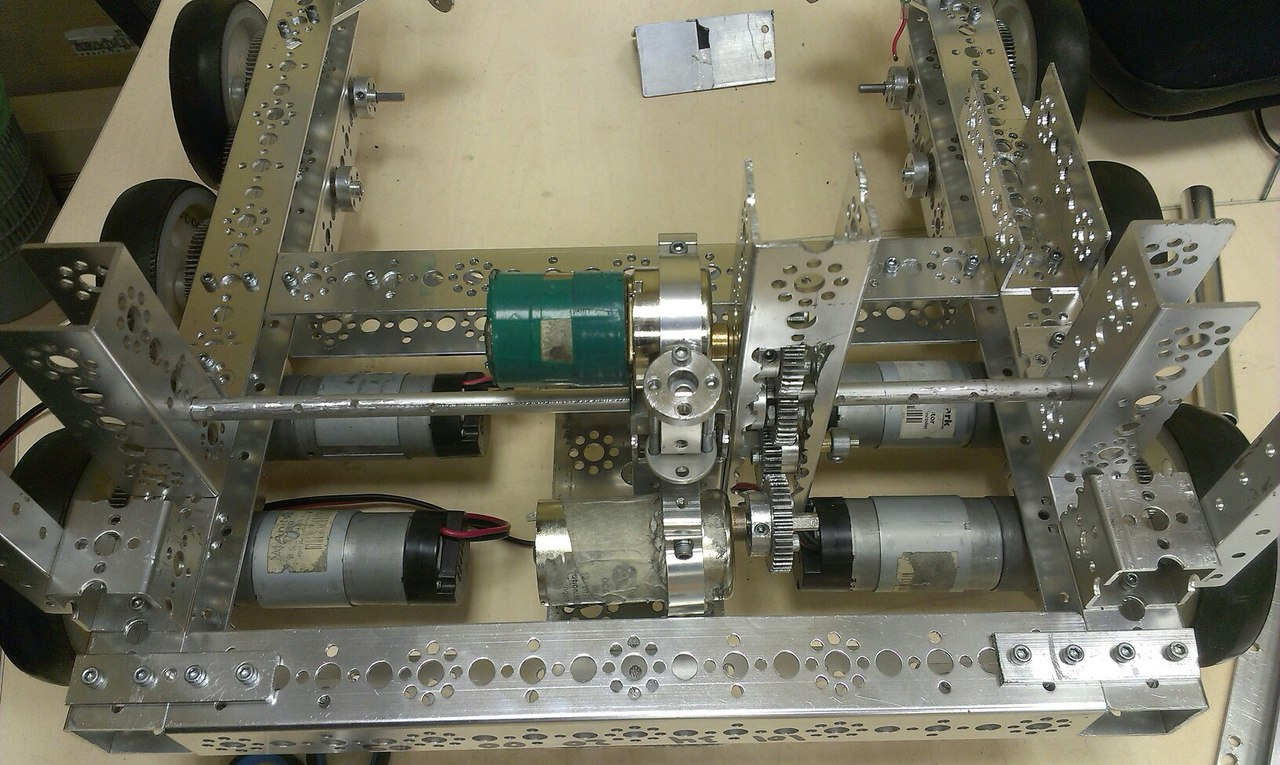
\includegraphics[scale=0.2]{3Engineering/5Team_meetings/days_of_meetings/2015.12.17/images/01}}
		\caption{Wheel base with 10cm wheels}
		\label{wheeel_base_10cm_wheels}
	\end{minipage}
\end{figure}

